Para la evaluaci\'on y comparaci\'on de los modelos entrenados con los
distintos hiperpar\'ametros se recurri\'o a las mismas m\'etricas que las
referidas en la secci\'on \ref{subsection-results-features} al evaluar
los posibles vectorizadores.
\par
En este caso, se encontr\'o que todos los modelos
entrenados con $penalty=None$ y
$class\_weight=\lbrace1:0.56,0:0.44\rbrace$\footnote{Los valores
reportados en el par\'ametros \texttt{class\_weight} corresponden a
las proporciones de cada clase halladas en el \textit{dataset}.}
arrojaron los mejores valores promedios considerando las cinco iteraciones
de la validaci\'on cruzada, sin importar el valor de $C$.
Las \'unicas excepciones a esto son el resultado en la
m\'etrica de precisi\'on y de cobertura. En la primera, el modelo entrenado con
$C=0.1$, $penalty=l2$ y $class\_weight=balanced$
obtiene un mejor resultado. No obstante, este modelo muestra uno de lo valores
m\'as bajos de cobertura y \textit{F1}. Es notable que, si bien tiene el mayor
valor de precisi\'on observado, esto no llega a compensar su bajo rendimiento
en la cobertura y de ah\'i que tambi\'en exhiba un valor bajo de \textit{F1}.
Y lo inverso sucede con la m\'etrica de cobertura, en la que el modelo
entrenado con $C=0.1$, $class\_weight=\lbrace1:0.56,0:0.44\rbrace$ y
$penalty=l2$ consigue el mejor rendimiento a costas de tener la peor precici\'on
observada.
Con valores m\'as moderados, los dem\'as modelos logran un mejor balance entre
\textit{precision} y \textit{recall} (ver tabla \ref{table-results-models-params}).

\begin{table}[h!]
    \centering
    \begin{adjustbox}{max width=\textwidth}
    \begin{tabular}{ *{7}{|c}| }
    \hline
    Par\'ametros & \textit{Accuracy} & Precisi\'on & Cobertura & \textit{F1} & \textit{F1-macro} & \textit{F1-weighted} \\
    \hline\hline
    $C=0.1, class\_weight=None, penalty=l2$ & 0.698 & 0.709 & 0.786 & 0.743 & 0.686 & 0.693 \\
    \hline
    $C=0.1, class\_weight=balanced, penalty=None$ & 0.710 & 0.733 & 0.762 & 0.742 & 0.701 & 0.706 \\
    \hline
    $C=0.1, class\_weight=balanced, penalty=l2$ & 0.679 & \cellcolor{highlight-blue!60}0.786 & 0.595 & 0.674 & 0.678 & 0.678 \\
    \hline
    $C=0.1, class\_weight=\lbrace1: 0.56, 0: 0.44\rbrace, penalty=None$ & \cellcolor{highlight-blue!60}0.717 & 0.728 & 0.797 & \cellcolor{highlight-blue!60}0.759 & \cellcolor{highlight-blue!60}0.706 & \cellcolor{highlight-blue!60}0.712 \\
    \hline
    $C=0.1, class\_weight=\lbrace1: 0.56, 0: 0.44\rbrace, penalty=l2$ & \cellcolor{highlight-orange!60}0.616 & \cellcolor{highlight-orange!60}0.607 & \cellcolor{highlight-blue!60}0.898 & 0.723 & \cellcolor{highlight-orange!60}0.541 & \cellcolor{highlight-orange!60}0.563 \\
    \hline
    $C=0.5, class\_weight=None, penalty=None$ & 0.710 & 0.739 & 0.752 & 0.741 & 0.703 & 0.708 \\
    \hline
    $C=0.5, class\_weight=None, penalty=l2$ & 0.648 & 0.715 & 0.628 & 0.665 & 0.644 & 0.647 \\
    \hline
    $C=0.5, class\_weight=balanced, penalty=None$ & 0.710 & 0.733 & 0.762 & 0.742 & 0.701 & 0.706 \\
    \hline
    $C=0.5, class\_weight=balanced, penalty=l2$ & 0.641 & 0.749 & 0.549 & 0.628 & 0.638 & 0.637 \\
    \hline
    $C=0.5, class\_weight=\lbrace1: 0.56, 0: 0.44\rbrace, penalty=None$ & \cellcolor{highlight-blue!60}0.717 & 0.728 & 0.797 & \cellcolor{highlight-blue!60}0.759 & \cellcolor{highlight-blue!60}0.706 & \cellcolor{highlight-blue!60}0.712 \\
    \hline
    $C=0.5, class\_weight=\lbrace1: 0.56, 0: 0.44\rbrace, penalty=l2$ & 0.679 & 0.682 & 0.808 & 0.735 & 0.657 & 0.667 \\
    \hline
    $C=1, class\_weight=None, penalty=None$ & 0.710 & 0.739 & 0.752 & 0.741 & 0.703 & 0.708 \\
    \hline
    $C=1, class\_weight=None, penalty=l2$ & 0.622 & 0.695 & 0.583 & 0.631 & 0.620 & 0.622 \\
    \hline
    $C=1, class\_weight=balanced, penalty=None$ & 0.710 & 0.733 & 0.762 & 0.742 & 0.701 & 0.706 \\
    \hline
    $C=1, class\_weight=balanced, penalty=l2$ & 0.622 & 0.739 & \cellcolor{highlight-orange!60}0.505 & \cellcolor{highlight-orange!60}0.598 & 0.620 & 0.617 \\
    \hline
    $C=1, class\_weight=\lbrace1: 0.56, 0: 0.44\rbrace, penalty=None$ & \cellcolor{highlight-blue!60}0.717 & 0.728 & 0.797 & \cellcolor{highlight-blue!60}0.759 & \cellcolor{highlight-blue!60}0.706 & \cellcolor{highlight-blue!60}0.712 \\
    \hline
    $C=1, class\_weight=\lbrace1: 0.56, 0: 0.44\rbrace, penalty=l2$ & 0.666 & 0.688 & 0.740 & 0.708 & 0.654 & 0.661 \\
    \hline
    $C=2, class\_weight=None, penalty=None$ & 0.710 & 0.739 & 0.752 & 0.741 & 0.703 & 0.708 \\
    \hline
    $C=2, class\_weight=None, penalty=l2$ & 0.629 & 0.717 & 0.560 & 0.624 & 0.626 & 0.626 \\
    \hline
    $C=2, class\_weight=balanced, penalty=None$ & 0.710 & 0.733 & 0.762 & 0.742 & 0.701 & 0.706 \\
    \hline
    $C=2, class\_weight=balanced, penalty=l2$ & 0.629 & 0.734 & 0.527 & 0.611 & 0.627 & 0.625 \\
    \hline
    $C=2, class\_weight=\lbrace1: 0.56, 0: 0.44\rbrace, penalty=None$ & \cellcolor{highlight-blue!60}0.717 & 0.728 & 0.797 & \cellcolor{highlight-blue!60}0.759 & \cellcolor{highlight-blue!60}0.706 & \cellcolor{highlight-blue!60}0.712 \\
    \hline
    $C=2, class\_weight=\lbrace1: 0.56, 0: 0.44\rbrace, penalty=l2$ & 0.647 & 0.689 & 0.673 & 0.678 & 0.641 & 0.646 \\
    \hline
\end{tabular}
\end{adjustbox}
\caption{Resultados obtenidos tras evaluar un modelo de Regresi\'on Log\'istica con
distintos hiperpar\'ametros. Los valores reflejan el rendimiento promedio de las
cinco iteraciones de la validaci\'on cruzada. Las celdas resaltadas en azul
corresponden a conjunto de hiperpar\'ametros que obtuvo un mejor rendimiento
promedio en cada m\'etrica de evaluaci\'on y las resaltadas en naranja, al
que obtuvo el peor rendimiento.}
\label{table-results-models-params}
\end{table}

Adicionalmente, se grafic\'o la media, el desv\'io est\'andar y el valor
obtenido en cada \textit{split} de la m\'etrica \textit{F1}
para los mejores 4 conjuntos de hiperpar\'ametros
(ver figura \ref{fig-results-features-fit-time})\footnote{Dado
que cuatro modelos presentaron el mismo rendimiento, se grafic\'o uno solo
de ellos para facilitar la visualizaci\'on}.
Aqu\'i podemos observar que los hiperpar\'ametros $C=1$, $penalty=None$
y $class\_weight=\lbrace1:0.56,0:0.44\rbrace$
presentan una media mayor y desv\'io menor que los otros
conjuntos, lo cual es consistente con el gr\'afico que muestra
los valores por iteraci\'on: si bien el modelo entrenado con estos hiperpar\'ametros
no logra superar en ning\'un \textit{split} al resto, tampoco exhibe
una variaci\'on tan grande y, en ning\'un caso, posee el peor valor
obtenido.
\par
Por cuestiones de simplicidad, dado que el c\'alculo de la intensidad inversa
de la regularizaci\'on se vuelve m\'as sencillo si se toma $C=1$ y que este es
adem\'as el valor tomado por la librería por defecto, se decide usar el conjunto
de hiperparámetros $C=1$, $penalty=None$ y
$class\_weight=\lbrace1:0.56,0:0.44\rbrace$ para entrenar el modelo final.
Para esta instancia, se usa el conjunto completo de datos de entrenamiento y luego
se lo eval\'ua con el \textit{held-out} separado para este fin. La tabla
\ref{table-results-models-held-out} muestra los resultados obtenidos en
esta evaluaci\'on y la figura \ref{fig-results-models-held-out}, la matriz
de confusi\'on.

\begin{figure}[h!]
    \centering
    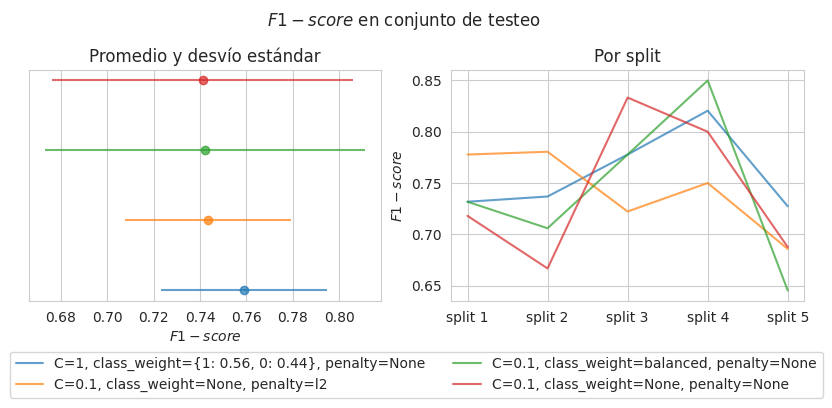
\includegraphics[scale=0.5]{../visualizations/parameters\_selection/f1_by_split.png}
    \caption{Resultados obtenidos al evaluar los distintos modelos con
    \textit{F1} durante la validaci\'on cruzada. El gr\'afico a izquierda muestra el
    promedio y el desvi\'o est\'andar de las cinco iteraciones para cada conjunto
    de hiperpar\'ametros y el gr\'afico de la derecha compara los valores obtenidos en
    cada iteraci\'on.}
    \label{fig-results-models-f1}
\end{figure}

\begin{figure}
    \begin{minipage}[b]{.6\linewidth}
    \centering
        \begin{adjustbox}{max width=\textwidth}
        \begin{tabular}{ *{5}{|c}| }
        \hline
        Clase & Precisi\'on & Cobertura & \textit{F1} & \textit{Soporte} \\
        \hline\hline
        0 (`en contra') & 0.93 & 0.78 & 0.85 & 18 \\
        \hline
        1 (`a favor') & 0.84 & 0.95 & 0.89  & 22 \\
        \hline\hline
        \textit{Accuray} & {--} & {--} & 0.78 & 40 \\
        \hline
        Promedio \textit{macro} & 0.89 & 0.87 & 0.88 & 40 \\
        \hline
        Promedio \textit{weighted} & 0.88 & 0.88 & 0.87 & 40 \\
        \hline
        \end{tabular}
        \end{adjustbox}
        \captionof{table}{M\'etricas de evaluaci\'on.}
        \label{table-results-models-held-out}
    \end{minipage}\hfill
    \begin{minipage}[t]{.35\linewidth}
      \centering
        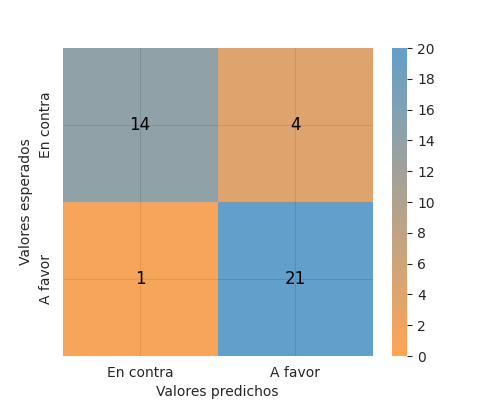
\includegraphics[scale=0.4]{../visualizations/models/confussion_matrix.png}
        \caption{Matriz de confusi\'on.}
        \label{fig-results-models-held-out}
    \end{minipage}
    \caption*{Resultados obtenidos a partir de entrenar un modelo de
    Regresi\'on Log\'istica con los mejores hiperpar\'ametros hallados
    ($C=1$, $penalty=None$ y $class\_weight=\lbrace1:0.56,0:0.44\rbrace$)
    y el conjunto completo de datos de entrenamiento,
    y luego evaluarlo con el \textit{dataset} de testeo.}
  \end{figure}

Se observa que el modelo final obtuvo un mejor \textit{accuracy} que sus
versiones pre{--}entrenadas durante la validaci\'on cruzada. Posiblemente
esto se deba al incremento de los datos durante el entrenamiento.
Mientras que, en la selecci\'on de hiperpar\'ametros, se entren\'o con $127$ discursos
y se teste\'o con $32$ en cada iteraci\'on; en la versi\'on final, el modelo fue entrenado
con $159$ documentos y evaluado con $40$. Este incremento no solo influye en
la cantidad y variabilidad de los datos que ve el modelo de regresi\'on sino
tambi\'en en el vectorizador, que se ve provisto de una mayor y m\'as diversa fuente
de informaci\'on para pesar las palabras presentes en los discursos y seleccionar
las $300$ m\'as representativas de ambas clases a predecir.
\par
Al comparar las m\'etricas de cobertura y precisi\'on en la tabla
\ref{table-results-models-held-out}, se puede inferir que el modelo posee
una leve tendencia a predecir mayormente discursos `a favor': la cobertura
de esta clase es mayor, pero su precisi\'on es menor; lo que indica que el modelo
predice mayormente esta clase aunque no en todos los casos acierta. Lo inverso
ocurre con los documentos `en contra'. Este fen\'omeno podr\'ia estar influido
por el hecho de tener clases levemente desbalanceadas y que sea la clase `a favor'
la mayoritaria, pese a que entre los hiperpar\'ametros seleccionados, se intentó
mitigar este desbalanceo.
\par
Por \'ultimo, se grafic\'o las $50$ palabras asociadas a los coeficientes positivos
y las $50$ asociadas a coeficientes negativos con mayor peso, aquellas que m\'as
fuertemente conducen a predicciones de la clase `a favor' y `en contra' respectivamente.
La figura \ref{fig-results-models-feature-importance} nos permite conjeturar qu\'e
\textit{tokens} caracterizan los discursos pertenecientes a ambas clases. Por el lado de los
discursos `a favor' se encuentran con \textit{tokens} como `mujer\_noun', `embarazo\_noun',
`sociedad\_noun', `salud\_noun', `aborto\_noun', `interrupción\_noun', `decidir\_verb',
`permitir\_voto', `derecho\_noun', `autonom\'ia\_noun', `respetar\_verb', `integral\_adj',
`muerte\_noun', `voluntaria\_adj'. Y, por el lado de los
documentos `en contra', se ven `madre\_noun', `vida\_noun', `ley\_noun', `norma\_noun',
`constituci\'on\_noun', `concepci\'on\_noun', `nacer\_verb',
`humano\_adj', `problema\_noun', `niña\_noun.

\begin{figure}[h!]
    \centering
    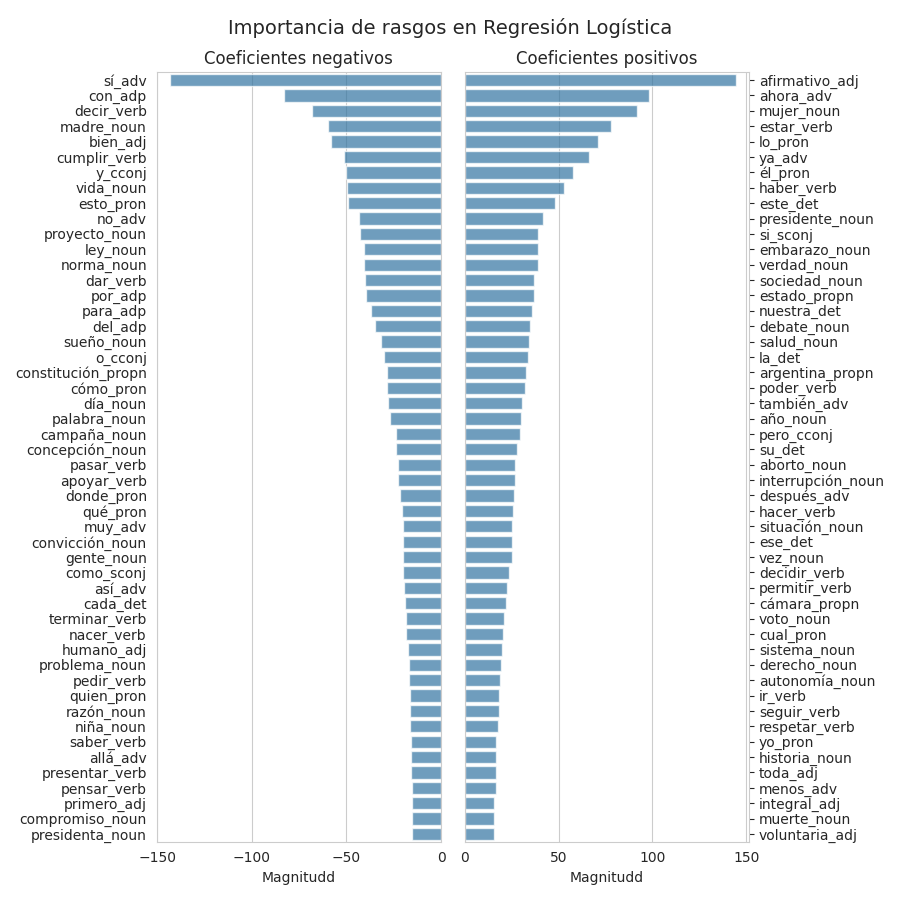
\includegraphics[scale=0.5]{../visualizations/models/lr_feature_importance_barplot_log_proba.png}
    \caption{Palabras asociadas a los coeficientes positivos y negativos con mayor peso.}
    \label{fig-results-models-feature-importance}
\end{figure}